\documentclass[12pt]{article}
\usepackage[margin=1in]{geometry}

% Start of preamble
%==========================================================================================%
% Required to support mathematical unicode
\usepackage[warnunknown, fasterrors, mathletters]{ucs}
\usepackage[utf8x]{inputenc}

% Always typeset math in display style
%\everymath{\displaystyle}

% Standard mathematical typesetting packages
\usepackage{amsmath,amssymb,amscd,amsthm,amsxtra, pxfonts}
\usepackage{mathtools,mathrsfs,dsfont,xparse}

% Symbol and utility packages
\usepackage{cancel, textcomp}
\usepackage[mathscr]{euscript}
\usepackage[nointegrals]{wasysym}

% Extras
\usepackage{physics}  % Lots of useful shortcuts and macros
\usepackage{tikz-cd}  % For drawing commutative diagrams easily
\usepackage{color}  % Add some color to life
\usepackage{microtype}  % Minature font tweaks
%\usepackage{pgfplots} % plots

\usepackage{enumitem}
\usepackage{titling}

\usepackage{graphicx}

% Common shortcuts
\def\mbb#1{\mathbb{#1}}
\def\mfk#1{\mathfrak{#1}}

\def\bN{\mbb{N}}
\def \C{\mbb{C}}
\def \R{\mbb{R}}
\def\bQ{\mbb{Q}}
\def\bZ{\mbb{Z}}
\def \cph{\varphi}
\renewcommand{\th}{\theta}
\renewcommand{\P}{\mathbb{P}}
\def \ve{\varepsilon}
\newcommand{\mg}[1]{\| #1 \|}

% Sometimes helpful macros
\newcommand{\floor}[1]{\left\lfloor#1\right\rfloor}
\newcommand{\ceil}[1]{\left\lceil#1\right\rceil}
\renewcommand{\qed}{\hfill\qedsymbol}

% Sets
\DeclarePairedDelimiterX\set[1]\lbrace\rbrace{\def\given{\;\delimsize\vert\;}#1}

% Some standard theorem definitions
\newtheorem{theorem}{Theorem}[section]
\newtheorem{corollary}{Corollary}[theorem]
\newtheorem{lemma}[theorem]{Lemma}

\theoremstyle{definition}
\newtheorem{definition}{Definition}[section]

\theoremstyle{remark}
\newtheorem*{remark}{Remark}

% End of preamble
%==========================================================================================%

% Start of commands specific to this file
%==========================================================================================%

\renewcommand{\ip}[2]{\langle #1, #2 \rangle}
\newcommand{\linf}[1]{\max_{1\leq i \leq #1}}
\newcommand{\seq}[2]{\qty(#1_#2)_{#2=1}^{\infty}}
\newcommand{\E}{\mathbb{E}}
\graphicspath{{./}}

\usepackage{hyperref}
\hypersetup{
	colorlinks=true,
	linkcolor=blue,
	filecolor=magenta,      
	urlcolor=cyan,
	pdftitle={Overleaf Example},
	pdfpagemode=FullScreen,
}

%==========================================================================================%
% End of commands specific to this file

\title{CSE 312 HW4}
\date{\today}
\author{Rohan Mukherjee}

\begin{document}
	\maketitle
	\begin{enumerate}[leftmargin=\labelsep]
		\item Our PMF will only take in values in the support of $X$, so $p_X(n) = 0$ for all $x$ that is not an integer between 1 and 10. By definition, $1/22=F_X(1) = \sum_{x \leq 1} p_X(x) = p_X(1)$, since $p_X(n) = 0$ for $n < 1$. Similarly, $1/11=F_X(2) = \sum_{x \leq 2} p_X(x) = p_X(1) + p_X(2)$, by the same reasoning, which tells us that $p_X(2) = 1/22$ again. Next, we see that $20/132=F_X(3) = p_X(1) + p_X(2) + p_X(3)$, by the same reasoning. Plugging in what we know gives us that $p_X(3) = 2/33$. Continuing in this way for the last 7 numbers in the support gives us $p_X(4) = 5/66$, $p_X(5) = 1/11$, $p_X(6) = 7/66$, $p_X(7) = 4/33$, $p_X(8)=3/22$, $p_X(9)=5/33$, and finally $p_X(10)=1/6$.
	
		\newpage
		\item \begin{enumerate}
			\item You can clearly get no 1s or 2s or all 1s or 2s. Also, if you move a 1 or 2 to a 3,4,5,6, then you BOTH have one less 1 or 2, AND another 3,4,5,6, so the difference would go down by 2 (e.g., 100 and 0, 99 and 1, 98 and 2, etc.). Since this could be done any number of times, the support is just $\set{-100, -98, -96, \ldots, 98, 100}$ (even integers in $[-100, 100]$). Or: let $n$ be the number of 1s and 2s. Then $100-n$ is the number of 3,4,5,6s. Then the number of 1s,2s minus the number of 3,4,5,6s is just $n-(100-n) = 2n-100$. Since $n \in [0, 100] \cap \bZ$, we see that this agrees with our answer from before.
			
			\item Let $Y = $ the number of 1s and 2s, and $Z = $ the number of 3,4,5,6s. I claim that $X = 4$, if and only if $Y=52$ and $Z = 48$. Clearly $Y + Z = 100$, since all dice rolls are either 1,2,3,4,5,6. Also, $X = 4$ says $Y-Z = 4$. The unique solution to this set of equations is $Y=52$ and $Z=48$ (the other direction is obvious). We are therefore looking for $\P(Y=52, Z=48)$. Thinking of the 100 rolls as a length 100 string, first pick the position of the 52 1s and 2s. There are ${100 \choose 52}$ ways to do this. Then assign each of the 52 spots either a 1 or a 2. This can be done in $2^{52}$ ways. Then, assign the remaining spots one of $3,4,5,6$, which can be done in $4^{48}$ ways. We see that $|Y=52, Z=48| = {100 \choose 52} \cdot 2^{52} \cdot 4^{48}$. Also, each roll can be anything from 1-6, and we are rolling 100 times, so the sample space has size $6^{100}$. We get that 
			\begin{align*}
				\P(Y=52, Z=48) = |Y=52, Z=48|/|\Omega| = \frac{{100 \choose 52} \cdot 2^{52} \cdot 4^{48}}{6^{100}}
			\end{align*}
		\end{enumerate}
	
		\newpage
		\item Let $X$ be the random variable profit. We are looking for $\E[X]$. Since the top 3 cards have either 0, 1, 2, or 3 diamonds, in each case we net $-1, z-1, 4,$ or 9 dollars respectively (the payout - the price to play), we see that the expected value of $X$ is just
		\begin{align*}
			\E[x] = 9 \cdot \P(X=9) + 4 \cdot \P(X=4) + (z-1) \cdot \P(X=z-1) + -1 \cdot \P(X = -1)
		\end{align*}
		Since the support of $X$ is just $\set{-1, z-1, 4, 9}$. $\P(X=9)$ is the probability of when the top three cards are all diamonds. Since the deck is shuffled uniformly, we only have to consider the top three cards. We need 3 of the 13 diamond cards to be on top, so we are looking for ${13 \choose 3}$ shuffles of the top 3 cards  out of the ${52 \choose 3}$ total possibilities for the top 3 cards. So $\P(X=9) = {13 \choose 3}/ {52 \choose 3}$. Similarly, if exactly two cards are diamonds, then we have to choose 2 of the 13 diamond cards to be in the shuffle, and then one of the 39 non-diamond cards, which can be done in ${13 \choose 2} \cdot 39$ ways. We see that $\P(X=4) = {13 \choose 2} \cdot 39 / {52 \choose 3}$. If exactly one card is diamond, we have to pick the diamond and then $2$ of the 39 non-diamond cards, which can be done in $13 \cdot {39 \choose 2}$ ways. We see that $\P(X=z-1) = 13 \cdot {39 \choose 2} / {52 \choose 3}$. Finally, if no cards are diamonds, we have to pick 3 of the 39 cards to be on the top, which can be done in ${39 \choose 3}$ ways. So $\P(X=-1) = {39 \choose 3} / {52 \choose 3}$. Plugging that $\E[X] = 0$ and these calculations into the above, we get
		\begin{align*}
			0 = 9 \cdot \frac{{13 \choose 3}}{{52 \choose 3}}+ 4 \cdot \frac{{13 \choose 2} \cdot 39}{{52 \choose 3}} + (z-1) \cdot \frac{13 \cdot {39 \choose 2}}{{52 \choose 3}} - \frac{{39 \choose 3}}{{52 \choose 3}}
		\end{align*}
		Solving this equation gives $z = \frac{310}{741}$. So if you only get 1 diamond you lose around 60 cents.
		
		\newpage
		\item 
		\begin{enumerate}
			Throughout this problem I will count the number of \textbf{socks}, NOT the number of pairs.
			\item Let $X$ be the total number of \textbf{pairs} of properly matched socks, and let \begin{align*}
				X_i = \begin{cases}
				1, \quad \text{the $i$th pair's left sock is paired with the right sock} \\
				0, \quad \text{else}
			\end{cases}
			\end{align*}
			There are 10 pairs of socks, so $1 \leq i \leq 10$. We see that the total number of pairs of properly matched socks can be found by starting at 0 and adding 1 precisely when a pairs left sock is paired with the right sock, so $X = \sum_{i=1}^{10} X_i$. We look to find the number of ways that the ith pair stays together. First, we need to find the total number of ways to pair up the socks. This can be done as follows: put all the left socks in a line. We want to find the number of ways we can assign right socks to these left socks. This can be done in $10!$ ways, since we are just permuting the right socks. Here is a picture:
			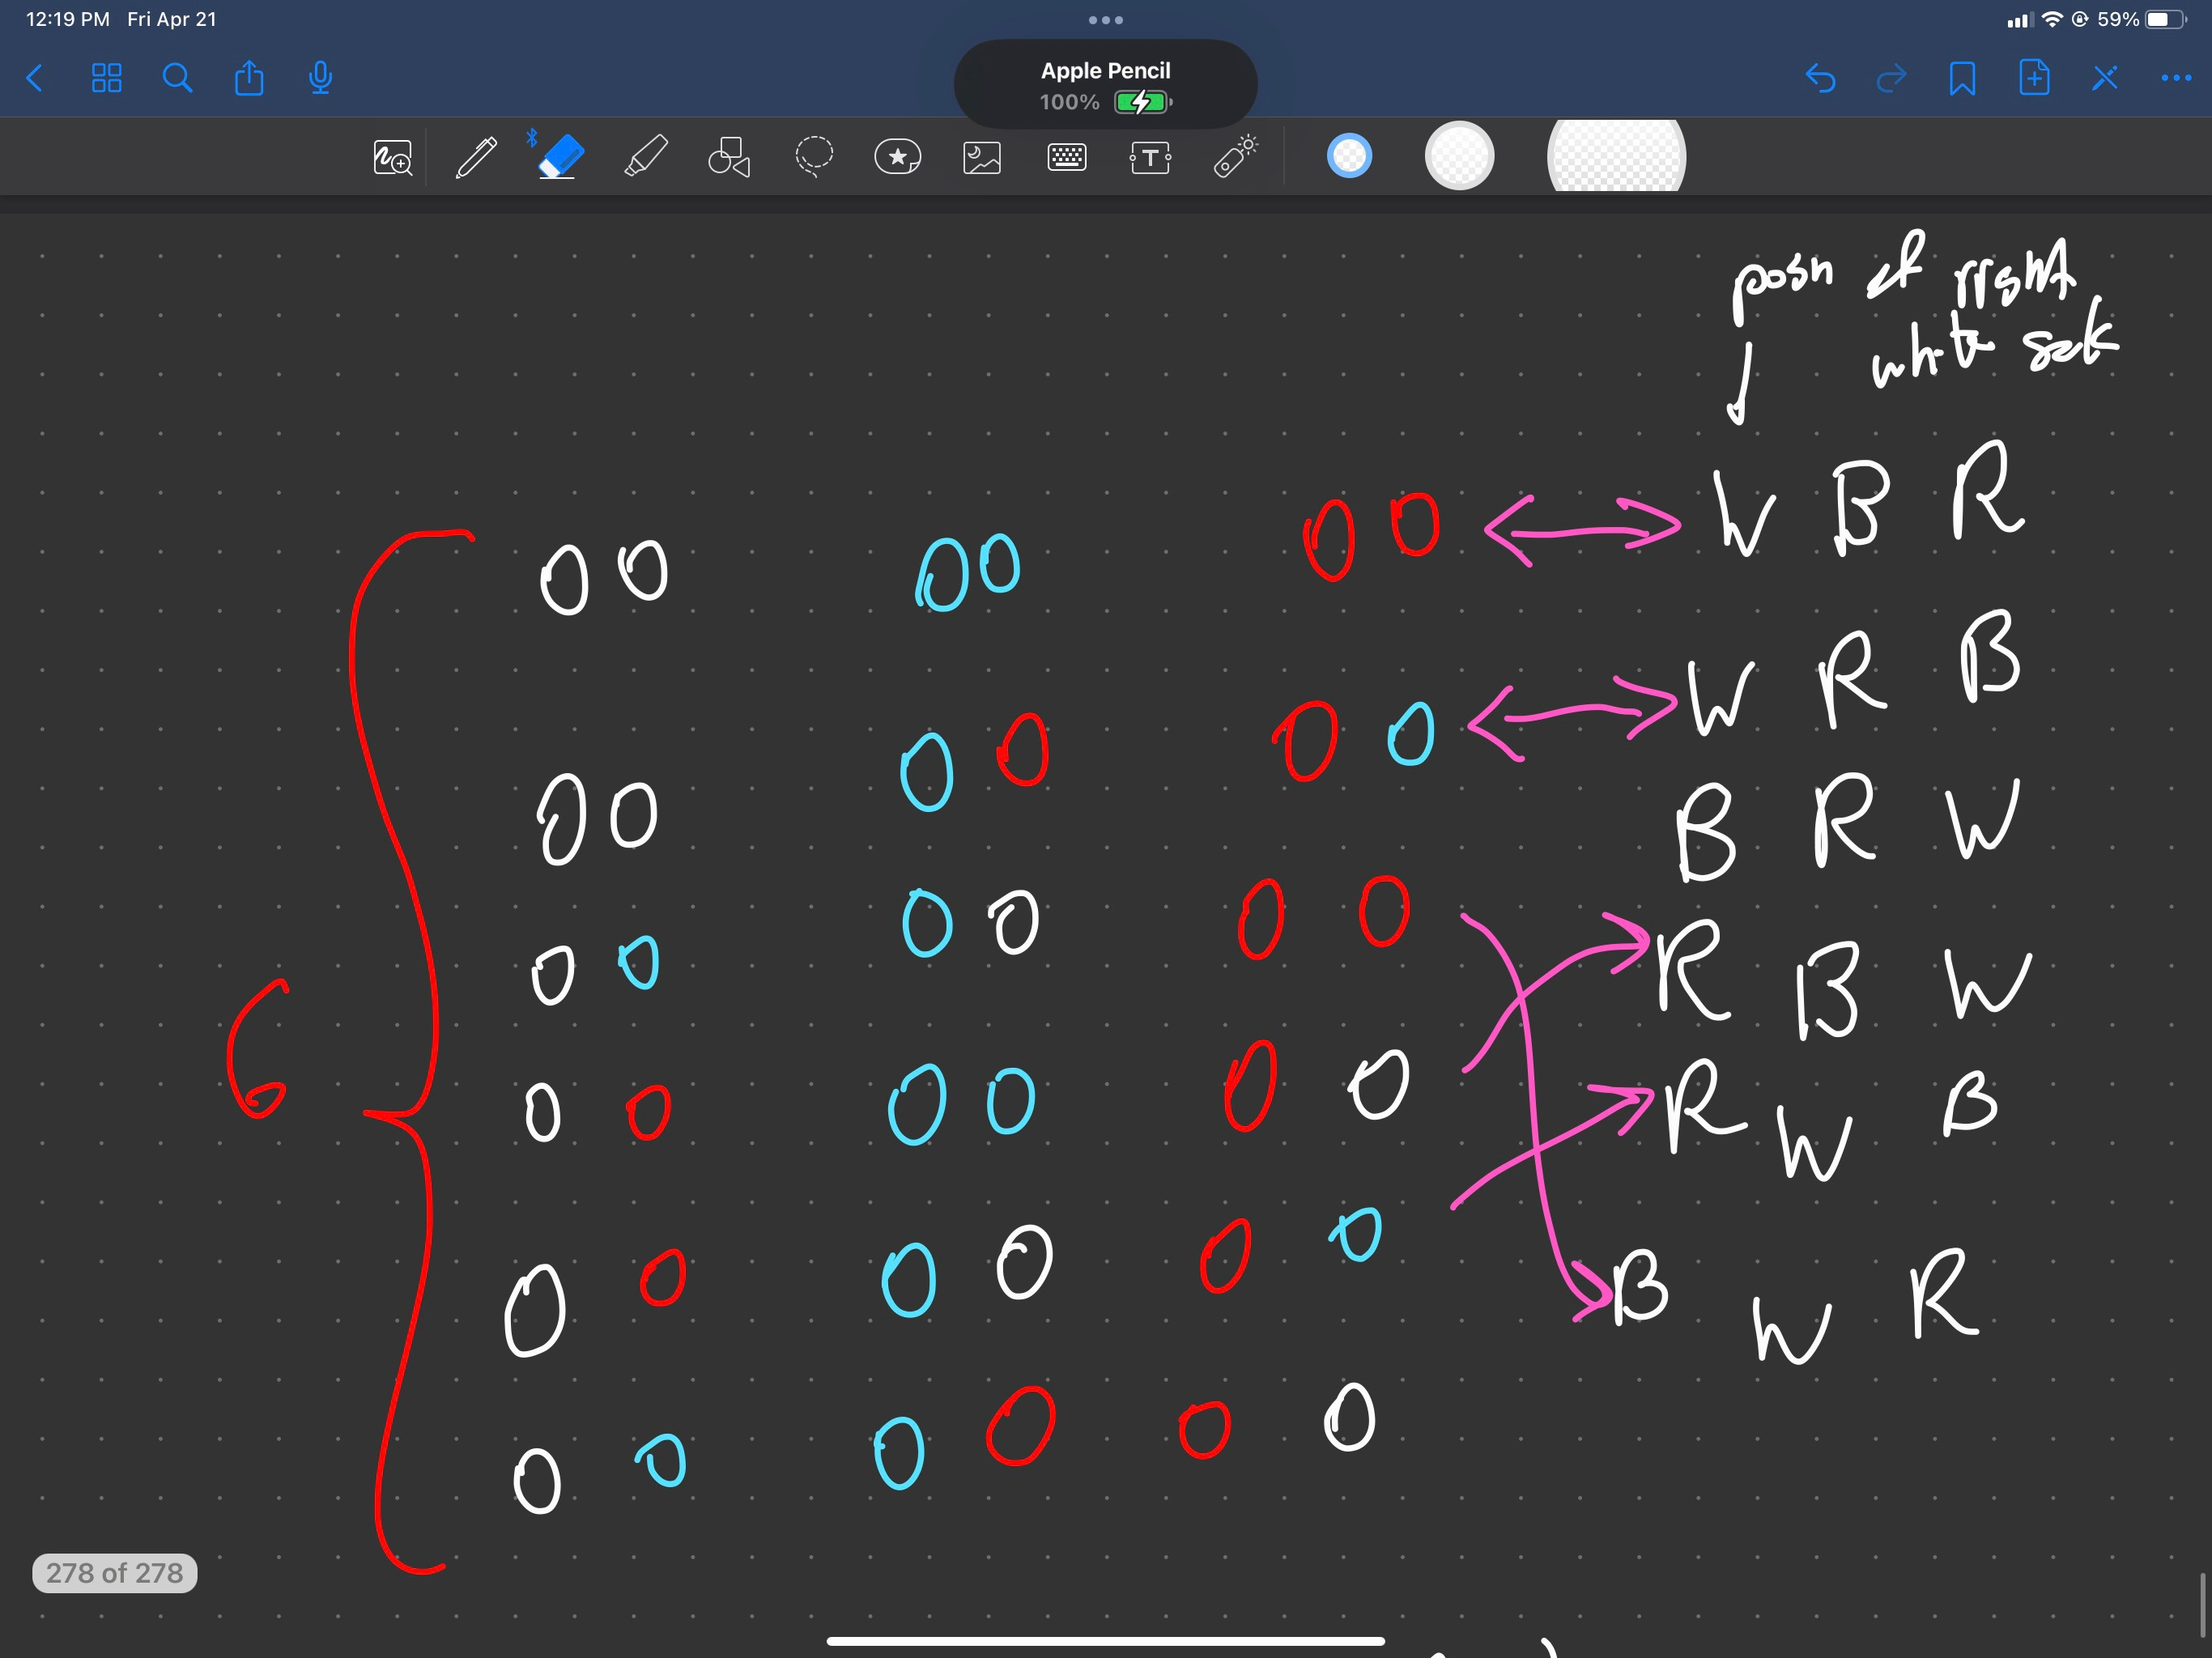
\includegraphics[width=\textwidth]{IMG_0084.jpeg}
			
			If we fix one pair of socks, i.e. if one pair of socks are properly matched, then we would be permuting the 9 other pairs, which can be done in $9!$ ways. So, we conclude that $\E[X_i] = 9!/10! = 1/10$, which makes intuitive sense, since we could also find this by fixing a left sock and saying it needs to be matched with 1 out of the 10 possible right socks. Since we have 10 pairs of socks, $\E[X] = \sum_{i=1}^{10} \E[X_i] = 10 \cdot 1/10 = 1$. Since there are two socks in a pair, $\E[\text{properly matched socks}] = 2 \cdot \E[X] = 2$.
			
			\item First, let $X = $ the number of left bright striped socks that are fashionably mismatched, $Y = $ the number of left checkered design socks that are fashionably mismatched, and $Z = $ the number of left solid socks that are fashionably mismatched. We first wish to calculate $\E[Y]$. I shall do this part slightly differently (but more intuitively) than the last part. Insight \#1: uniformly pairing socks together is just pairing left socks with right socks from any of the pairs. Insight \#2: Therefore, we just have to consider left socks that are fashionably mismatched, and then double the answer (since if a pair is fashionably mismatched, there are really two socks in the pair). This tells us that $\E[\text{number of fashionably mismatched socks}] = 2\E[X + Y + Z]$.
			
			Let $X_i = $ the $i$th left bright striped sock is fashionably mismatched. Clearly $X = \sum_{i=1}^3 X_i$. We wish to find the probability that the right sock assigned to the $i$th bright striped left sock is another bright striped sock not in the same pair. Since there are $3-1=2$ right bright striped socks not in the $i$th pair, and a total of $10$ socks we could assign to be it's right sock, this has a probability of $1/5$ of happening. We see that $\E[X_i] = 1/5$ for all $1 \leq i \leq 3$. Therefore, $\E[x] = 3/5$. Similarly, letting $Y_i = $ the $i$th left checkered design sock is fashionably mismatched ($i \leq 1 \leq 5$). This time, there are $5-1$ right checkered socks not in the $i$th pair, and there are still 10 possible right socks, so $Y_i$ has a probability equal to $4/10 = 2/5$ of happening. Therefore, $\E[Y] = 5 \cdot 2/5 = 2$. The same logic will give us $\E[Z] = 2 \cdot 1/10 = 2/10$. We conclude that $\E[X+Y+Z] = \E[X] + \E[Y] + \E[Z] = 3/5 + 1/5 + 2 = 4/5 + 2$. We have to double this as we discussed above, so we conclude that $\E[\text{number of fashionably mismatched socks}] = 8/5 + 4$.
		\end{enumerate}
		
		\newpage
		\item 
		\begin{enumerate}
			\item Let $X=$ the number of 4-flavor syrup combinations that taste good. There are ${n \choose 4}$ syrup combinations. Line them up, and let $X_i = $ the $i$th syrup combination tastes good ($1 \leq i \leq {n \choose 4}$). It is now clear that $X = \sum_{i=1}^{n \choose 4} X_i$ (running through all syrup combinations, adding a 1 if it tastes good, and adding nothing if it doesn't).
			
			\item
			We see that
			\begin{align*}
				\E[X] = \sum_{i=1}^{n \choose 4} \E[X_i]
			\end{align*}
			An arbitrary syrup combination of 4 syrups will taste good if and only if all pairs of syrup combinations in the 4-combination taste good. There are ${4 \choose 2}$ pairs in any 4-combination. Line them up again, the probability that the syrup combination tastes good is going to be the probability that the first pair tastes good * the probability the second pair tastes good and so on. Since there are ${4 \choose 2}$ pairs, and each pair has probability $p$ of tasting good, we see that the probability that the 4-combination tastes good is just $p^{4 \choose 2} = p^6$. Plugging this back into our formula gives us $\E[X] = \sum_{i=1}^{n \choose 4} p^6 = {n \choose 4}p^6$. My mind is blown!!! Linearity of expectation is awesome.
		\end{enumerate}
		
		\newpage
		\item Let $X = $ the number of maximal runs, and let \begin{align*}
			X_i = \begin{cases}
				1, \quad \text{coin at $i$th position $\neq$ coin at $i+1$th position} \\
				0, \quad \text{else}
			\end{cases}
		\end{align*}
		for $1 \leq i \leq n-1$. I claim that $X = \sum_{i=1}^{n-1} X_i + 1$. Lets look at an example. If we had $HHTT$, we would get $X_1 = 0$, $X_2 = 1$, and $X_3 = 0$. The maximal number of runs is $2$, which is certainly equal to $X_1 + X_2 + X_3 + 1$. The $+1$ at the end comes in because we always exclude the last run--if the last character is different from the one before it, then it will never be considered, and if it equals the one before it, that length $\geq 2$ run will never get added since there is no indicator on the last coin. The idea is that the number of maximal runs can be counted by the number of times the string changes from H to T, and vice versa, and then adding 1 to the end because we excluded it. We now wish to find $\E[X_i]$. Let $Y_i = $ coin at $i$th position $\neq$ coin at $i+1$th position. We know that $\E[X_i] = \P(Y_i)$. By the law of total probability, $\P(Y_i) = \P(Y_i \mid \text{$i$th position is heads}) \cdot \P(\text{$i$th position is heads}) + \P(Y_i \mid \text{$i$th position is tails}) \cdot \P(\text{$i$th position is tails})$. If the $i$th position is heads, for $Y_i$ to happen the $i+1$th position would need to be tails. This happens with probability $1-p$, so $\P(Y_i \mid \text{$i$th position is heads})=1-p$. $\P(\text{$i$th position is heads}) = p$, as the problem states. Similarly, if the $i$th position is tails, the next position would need to be heads, which happens with probability $p$. The probability of getting tails in the $i$th position is just $1-p$. We conclude that $\P(Y_i) = 2p(1-p)$. Plugging this in, we get
		\begin{align*}
			\E[X]=\E\qty[\sum_{i=1}^{n-1} X_i+1] &= \qty(\sum_{i=1}^{n-1} \E[X_i]) + 1 \\
			&= \qty(\sum_{i=1}^{n-1} 2p(1-p)) + 1 \\
			&= 2(n-1)p(1-p) + 1
		\end{align*}
		What an amazing question!!! Such an elegant solution!!!
		
		\newpage
		\item[7.1.1.]
		\begin{enumerate}
			\item The prosecutor is talking about $\P(\overline{G} \mid T)$.
			
			\item The false positive rate--i.e., given that you are innocent, the probability you test positive--is therefore $\P(T \mid \overline{G})$.
			
			\item The prosecutor is describing $\P(\overline{G} \mid T)$ in his argument, stating that it is $\frac{1}{10,000,000}$, while the actual numbers tell us that $\P(T \mid \overline{G}) = \frac{1}{10,000,000}$--which is separate from what he he is talking about. So he is talking about one probability and citing a different one.
		\end{enumerate}
		\item[7.1.2.]
		\begin{enumerate}
			\item We are trying to analyze the probability that the defendant is guilty given the test shows up positive, so prior to running the test we are trying to analyze the probability is guilty. I.e., we are looking for $\P(G)$. Since exactly one person committed the crime, and there are 330,000,000 people in the country, $\P(G) = \frac{1}{330,000,000}$.
			
			\item We see that (by Bayes rule and the LTP)
			\begin{align*}
				\P(G \mid T) = \frac{\P(T \mid G) \cdot \P(G)}{\P(T \mid \overline{G}) \cdot \P(\overline{G}) + \P(T \mid G) \cdot \P(G)}
			\end{align*}
			We showed above that $\P(T \mid \overline{G}) = \frac{1}{10,000,000}$. The false negative rate is: given that the person is guilty, what is the probability the test answers negative, i.e. it is $\P(\overline{T} \mid G)$. We see that this equals $1 - \P(T \mid G)$. So $\P(T \mid G) = 1 - \P(\overline{T} \mid G) = \frac{99,999,999}{100,000,000}$.
			
			Also, $\P(\overline{G}) = \frac{329,999,999}{330,000,000}$. Plugging these all in gives us
			\begin{align*}
				\P(G \mid T) = \frac{99,999,999}{3,399,999,989}
			\end{align*}
			which is indeed about $1/34$ (to like 7 decimal places!).
		\end{enumerate}
	
		\item[7.2]
		\begin{enumerate}
			\item  My first idea is that there is a VERY likely chance that the guilty lives in the seattle area--so we can restrict ourselves to just the seattle area. That means that the probability that a random person from seattle is guilty, i.e. $\P(G) = \frac{1}{4,000,000}$. This would mean that $\P(\overline{G}) = \frac{3,999,999}{4,000,000}$. I won't incorporate the first bullet point--so the false negative/positive rates will stay the same from the last question. If we only test people in Seattle, assuming the criminal lives in Seattle,
			\begin{align*}
				\P(G \mid T) = \frac{\P(T \mid G) \cdot \P(G)}{\P(T \mid \overline{G}) \cdot \P(\overline{G}) + \P(T \mid G) \cdot \P(G)}
			\end{align*}
			Once again $\P(T \mid G) = \frac{99,999,999}{100,000,000}$, and $\P(T \mid \overline{G}) = \frac1{10,000,000}$. Plugging these new values in,
			$\P(G \mid T) = \frac{33,333,333}{46,666,663}$ which is around 71.43\%, which is MUCH higher. Now I can see why the number of 9's matters! If we restrict the guilty to 2 order of magnitudes smaller, then it turns out to be a much better estimate.
			
			\item Since I didn't end up using the first bullet point, a limitation of my argument is that the DNA samples from the FBI are only criminals. This \textit{could} affect the false positive/negative rate for testing random people in the Seattle metro area that aren't criminals (e.g., maybe the FBI has more of their DNA because they are repeat offenders, which would effect the false positive/negative rates because they have more samples to test against, and also would have the denominators be MUCH smaller, which would probably make the number from part (a) smaller). So I would've liked to know the false positive/negative rate among random (non-criminals included) people living in JUST the Seattle Metro area, not the whole country.
		\end{enumerate}
	
		\item[7.3]
		\begin{enumerate}
			\item Let $C=$ the student cheated on the exam, and $O=$ their camera was off.
			\item I looked for a while, and I couldn't find a study that gave $\P(O \mid C)$. However, I think if you are cheating, then it is REALLY likely that you have your camera off. \href{https://onlinelibrary.wiley.com/doi/full/10.1002/ece3.7123#:~:text=The%20vast%20majority%20of%20students,several%20reasons%20for%20doing%20so.}{this} says that 90\% of students kept their camera off at some time during online learning, but not necessarily during a test. Since I couldn't find anything else, I will take $\P(O \mid C) = 0.9$ (this seems pretty reasonable, if you are cheating, there is a very good chance you have your camera off). \href{https://www.ncbi.nlm.nih.gov/pmc/articles/PMC10019462/}{this} link shows that 60\% of students admitted to cheating during online exams most of the time. We shall take this number to mean $\P(C)$. Finally, we want to find $\P(O)$. \href{https://chsktr.com/2876/entertainment/cameras-off/}{this} article claims that ``59.8\% of students claimed they keep their camera off routinely during zoom classes''. We shall take that number to mean $\P(O)$. We can therefore conclude that,
			\begin{align*}
				\P(C \mid O) = \frac{\P(O \mid C) \P(C)}{\P(O)} = \frac{0.9 \cdot 0.6}{0.598} \approx 0.90301
			\end{align*}
			This tells us that the probability a student is cheating on an exam, given their camera is off, is around 90\%.
			
			
			\item I find this calculation pretty interesting--IF you have your camera off, it is VERY likely you are cheating on an exam. I honestly do think this number is pretty likely since the percentage of people cheating online is insanely high. For an interesting side note, I found an article that talked about cheating on AP tests, and it showed the google search results of common words like ``integral, derivative, etc.'' Unsurprisingly, those words were searched up a LOT during the day of the AP Calc test, it was a jump of like 1000\%! 
			
			\item A huge limitation is that these numbers were found from different articles, because no one article really talked about cheating and specifically looking at the camera being off (At least, in the 30 mins - hour that I looked online I couldn't find it). Also, the sample sizes for some of the studies was quite small--one study had a sample size of less than 300, which would generate an error of around $1/\sqrt{300}$ which is about 5\%. This could change the final probability, but it would still be pretty large. Also, the largest limitation is that I couldn't find any source detailing $\P(O \mid C)$, so I just had to reasonably estimate it.
		\end{enumerate}
	\end{enumerate}
\end{document}
